\documentclass[tikz]{standalone}
\begin{document}

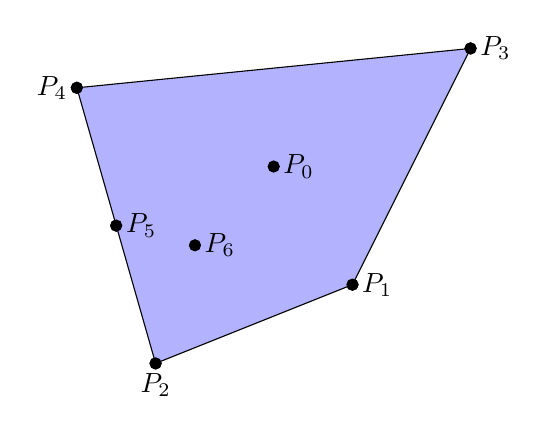
\begin{tikzpicture}

    \filldraw[black] (0.5, 0) coordinate(p0) circle (2pt) ;
    \filldraw[black] (1.5,-1.5) coordinate(p1) circle (2pt) ;
    \filldraw[black] (-1,-2.5) coordinate(p2) circle (2pt) ;
    \filldraw[black] (3,1.5) coordinate(p3) circle (2pt) ;
    \filldraw[black] (-2,1) coordinate(p4) circle (2pt) ;
    \filldraw[black] (-1.5,-0.75) coordinate(p5) circle (2pt);
    \filldraw[black] (-0.5,-1) coordinate(p6) circle (2pt);
    
  
    \fill[blue!30] (p3) -- (p1) -- (p2) -- (p4) -- cycle;

    \draw (p3) -- (p1) -- (p2) -- (p4) -- cycle;

    \filldraw[black] (0.5, 0) coordinate(p0) circle (2pt) node[right] {$P_0$};
    \filldraw[black] (1.5,-1.5) coordinate(p1) circle (2pt) node[right] {$P_1$};
    \filldraw[black] (-1,-2.5) coordinate(p2) circle (2pt) node[below] {$P_2$};
    \filldraw[black] (3,1.5) coordinate(p3) circle (2pt) node[right] {$P_3$};
    \filldraw[black] (-2,1) coordinate(p4) circle (2pt) node[left] {$P_4$};
    \filldraw[black] (-1.5,-0.75) coordinate(p5) circle (2pt) node[right] {$P_5$};
    \filldraw[black] (-0.5,-1) coordinate(p6) circle (2pt) node[right] {$P_6$};
    
    
  
  
\end{tikzpicture}

\end{document}